\documentclass{article}
\usepackage[utf8]{inputenc}
\usepackage{amsmath}
\usepackage{graphicx}


\title{NA HW2}
\author{Christian Lascsak 013763742}
\date{November 2020}

\begin{document}

\maketitle

\section{Paper and Pencil Exercises}
\subsection{First}
We have discussed elementary elimination matrices Mk in class. Prove the
following two properties of elementary elimination matrices, which are very important for
making LU factorization work efficiently in practice:

\par\noindent
Property (a): Mk is nonsingular.
Hint: Represent \(M_k^{-1}\)
explicitly and then show that \(M_k M_k^{-1} = M_k^{-1} M_k = I\)
\par
\noindent
practice:
Property (b): The product of two elementary elimination matrices \(M_k\) and \(M_j\) with \(k \leq j\) is essentially their “union”; and therefore they can be multiplied without any computational
cost.
\par\noindent
Assuming we have a 2x2 elimination Matrix 
\begin{equation}
    M_k^{-1} =
    \left( 
    \begin{array}{rrrr}
    1 & 0 & 0\\
    -2 & 1 & 0\\
    1 & 0 & 1\\
    \end{array}\right)
\end{equation}

\begin{equation}
    det(M) = \begin{vmatrix}
    1 & 0 & 0\\
    -2 & 1 & 0\\
    1 & 0 & 1\\
    \end{vmatrix} = 1*1*1 + 0*0*1 + 0*(-2)*0 - 1*1*0 - 0*0*1 = 1
\end{equation}

\par\noindent
The determinant is 1, which means, that this matrix is non-singular. So for \(M\) there exists an \(M^{-1}\)

\begin{equation}
    M * M^{-1} = I
\end{equation}
Therefore 
\begin{equation}
    M^{-1} =  \left( \begin{array}{rrrr}
    1 & 0 & 0\\
    2 & 1 & 0\\
    -1 & 0 & 1\\
    \end{array}\right)
\end{equation}
     
\par\noindent

\subsection{Part1 - A Condition Estimator}
The condition number of a matrix describes the ratio of the maximum to minimum stretching of a vector by a matrix. That's the reason why a matrix with a \(|M| = 0\)  has a condition number of infinity.
Only a matrix with a range of infinity for stretching and minimizing a vector, can minimize it to zero. Therefore making the matrix singular.
\par\noindent
The Calculation of the condition number is:
\(K(A) = ||A|| * ||A^{-1}||\).
\par\noindent
However the calculation of \(||A^{-1}||\) is very expensive. This is because of the complexity for calculating the inverse of a Matrix ($O(n^3)$ for Gauss Jordan Elimination).
There are other algorithms out there, however they are all more complex than $O(n^2)$.
This makes the idea to estimate  \(||A^{-1}||\) very attractive. For doing this we need a few steps.
Firstly, we would solve a linear system \(A z = y\).
The resulting z and y can then be used to estimate the normed inverse of A: \(\\||A^{-1}|| = \frac{||z||}{||y||}\).
But the problem here is, what is y? 
There are few methods to calculate y. One is to simply generate a random y - so that \(\frac{||z||}{||y||}\) is as big as possible.
However, the other method is to make an LU decomposition of A 
\begin{equation}
    A = L U
\end{equation}
and then solve 
\begin{equation}
    U^T w = e
\end{equation}
With that we can then solve 
\begin{equation}
    L^T y = w
\end{equation}
generating a \(y\) for our estimation.

\subsection{Part 2 -  Average Case Perturbation Errors}
For Part 2 we are generating random perturbation Errors E and \(\Delta b\) - with a norm of \(10^{-8}\).
This can be achieved by generating a random Matrix, dividing its components by its first norm and then multiplying it by the desired norm \(10^{-8}\).
\begin{equation}
     E := (E / ||E||_1) * 10^{-8}
\end{equation}
We do the same for \(\Delta b\) (the error of b) in \(A x = b\).
\begin{equation}
     \Delta b := (\Delta b / ||\Delta b||_1) * 10^{-8}
\end{equation}
\par\noindent
Then we calculate the solution x of \(A x = b\). \^x is also calculated, by solving the linear system including the perturbation:
\begin{equation}
    (A + E)  \^x =  (b + \Delta b);
\end{equation}
With \^x we can then calculate: \(\Delta x = \^x-x\)
\begin{figure}
    \centering
    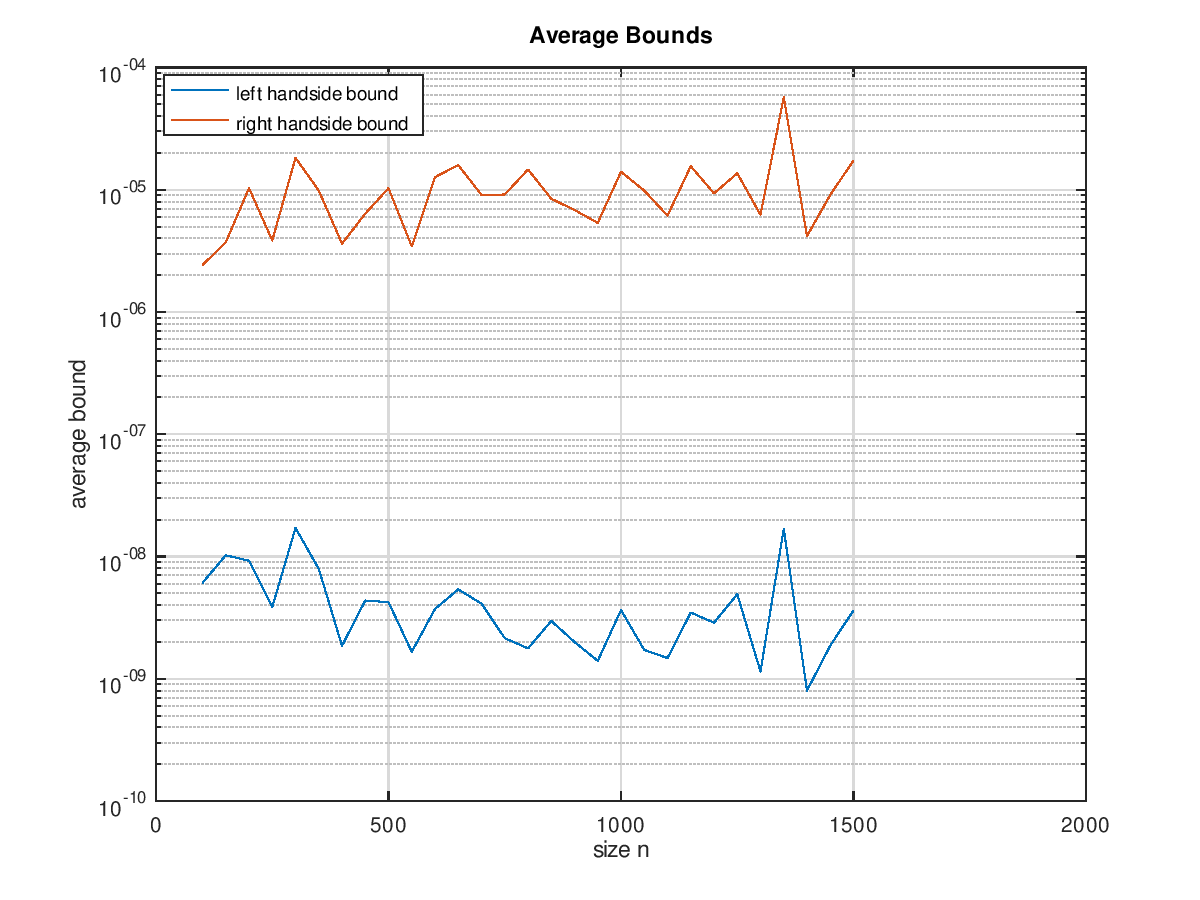
\includegraphics[width=0.8\textwidth]{part2_img.png}
    \caption{The comparison of the left hand-side error bound and the right hand-side error bound on a logarithmic scale}
    \label{fig:part2_result}
\end{figure}
We now have all the components for calculating the lower (left side) and the upper bound (right side):

\begin{equation}
    \frac{||\Delta x||}{||x||} \leq cond(A) (\frac{||\Delta b||}{||b||} + \frac{||E||}{||A||})
\end{equation}

\par\noindent
Calculating the bounds for many A and averaging the results gives us the following graph(\ref{fig:part2_result}).
We can see that the higher n is (which means the more dimensions the linear system has), the more space is between the lower and the upper bound.
This means, that the perturbation increases with the size of A.

\end{document}
